\documentclass[10pt, twocolumn]{article}

\usepackage{amsmath, amssymb, amsthm}
\usepackage{graphicx}
\usepackage{booktabs}
\usepackage{algorithm}
\usepackage{algorithmic}
\usepackage[margin=1in]{geometry}
\usepackage{hyperref}
\usepackage{natbib}
\usepackage{xcolor}
\usepackage{caption}

\newtheorem{proposition}{Proposition}
\newtheorem{theorem}{Theorem}
\newtheorem{corollary}{Corollary}
\newtheorem{definition}{Definition}

\title{Adaptive and Proactive Multi-Agent Coordination as Constrained DAG Scheduling\\with Error Propagation Control}

\author{%
  Anonymous Authors\\
  \textit{Under Review}
}

\date{}

\begin{document}
\maketitle

% ─────────────────────────────────────────────────────────────────────────────
\begin{abstract}
Multi-agent systems for complex task execution are typically orchestrated with open-loop strategies that react only after coordination errors have already propagated. We formalize multi-agent coordination as constrained DAG scheduling with error propagation and study both reactive decisions (assignment, validator placement, representation choice) and proactive controls (speculation, early stopping, skipping, and pre-warming). We derive analytical results for critical-path-first assignment, greedy single-validator placement, cube-root agent-count scaling, and a speculation hit-rate threshold $\rho^*$ on serial chains. We then propose an adaptive controller that replans unfinished work and augments it with interface-aware proactive controls. In simulation, the reactive stack reduces mean total cost by 42\% versus a naive round-robin baseline, while a heuristic proactive stack---with parameters tuned on the same DAG family---reduces cost by up to 18\% over the adaptive controller with representation selection; serial-chain experiments show an empirical speculation crossover near $\rho^* \approx 0.55$--$0.70$.
\end{abstract}

% ─────────────────────────────────────────────────────────────────────────────
\section{Introduction}

Multi-agent systems powered by large language models (LLMs) are increasingly deployed for complex, multi-step tasks such as software engineering, research synthesis, and data analysis \citep{yao2023react, hong2023metagpt, wu2023autogen}. These systems decompose a high-level goal into subtasks executed by specialized agents. Despite their growing adoption, coordination in these systems remains largely ad hoc: agents are assigned to tasks without consideration of the critical path, errors propagate unchecked across agent boundaries, and the communication format between agents is chosen without regard to its effect on downstream error amplification.

We identify three coupled subproblems that any multi-agent orchestrator must solve:
\begin{enumerate}
    \item \textbf{Assignment}: Which agent executes which task?
    \item \textbf{Scheduling}: In what order, given the dependency structure?
    \item \textbf{Coordination}: What communication topology and representation format minimize overhead while controlling error propagation?
\end{enumerate}

Current frameworks solve these independently or not at all. Round-robin assignment ignores the critical path. Fixed communication topologies ignore the dependency structure of the problem. Most critically, error propagation---the amplification of mistakes as outputs pass from one agent to the next---is a first-order concern that is universally ignored.

Reactive replanning addresses only part of this problem. By the time a controller observes a bad handoff, it has already paid at least one serial dependency and one context transfer. In realistic LLM workflows, however, earlier signals are often available: downstream tasks can sometimes begin from a structured sketch before upstream content is finalized; partial outputs reveal quality trends before a task completes; high-quality intermediates can make downstream verification tasks redundant; and likely future handoffs can be pre-warmed with cheap anticipatory context. These proactive controls are standard intuitions in other systems domains, but they are mostly absent from current agent orchestration abstractions.

\paragraph{Contributions.}
\begin{enumerate}
    \item A formal framework casting multi-agent coordination as constrained optimization over a task DAG with error propagation (Section~\ref{sec:formulation}).
    \item Analytical results on critical-path assignment dominance, optimal validator placement, optimal agent count scaling, multiplicative error bounds, and the speculation hit-rate threshold on a serial critical path (Section~\ref{sec:analytical}).
    \item An adaptive closed-loop orchestration policy augmented with four proactive control primitives: speculative execution, predictive early stopping, conditional DAG morphing, and context pre-warming (Section~\ref{sec:policy}).
    \item A mechanistic simulation study over seven experimental settings that stress-tests both reactive and proactive controls under stylized but reproducible conditions (Section~\ref{sec:experiments}).
\end{enumerate}

% ─────────────────────────────────────────────────────────────────────────────
\section{Problem Formulation}
\label{sec:formulation}

\subsection{Task DAG Model}

A goal $G$ decomposes into a task DAG $\mathcal{T} = (V, E)$ where $V = \{t_1, \ldots, t_n\}$ are tasks with duration $d_i$ and failure probability $p_i$, and $E$ encodes dependencies: $(t_i, t_j) \in E$ means $t_j$ cannot start until $t_i$ completes. An agent set $\mathcal{A} = \{a_1, \ldots, a_k\}$ is available, each with speed multiplier $s_k$ (effective duration $d_i / s_k$).

\subsection{Decision Variables}

We optimize over four coupled variables:
\begin{itemize}
    \item \textbf{Assignment matrix} $X \in \{0,1\}^{n \times k}$ with $\sum_k x_{ik} = 1$: each task is assigned to exactly one agent.
    \item \textbf{Adaptive policy} $\pi$: a state-dependent re-assignment rule.
    \item \textbf{Communication topology} $\mathcal{G}$: the subgraph of inter-agent communication edges.
    \item \textbf{Representation format} $R = \{r_{ij}\}$: the encoding format at each handoff edge.
\end{itemize}

\subsection{Objective Function}

\begin{multline}
\label{eq:objective}
\min_{X, \pi, \mathcal{G}, R} \; \mathbb{E}_\pi\!\left[\text{makespan}\right] \\
  + \alpha \!\sum_{(i,j) \in \mathcal{G}}\! \text{OH}(a_{x_i} \!\to\! a_{x_j}, r_{ij})
  + \beta \sum_i \epsilon_i
\end{multline}

where the three terms capture latency, coordination overhead, and accumulated error respectively. The weights $\alpha, \beta > 0$ trade off these objectives.

\subsection{Critical Path Analysis}

The earliest start and finish times are computed via topological dynamic programming:
\begin{align}
    \text{est}(t_i) &= \max_{t_j \in \text{pred}(t_i)} \text{eft}(t_j), \\
    \text{eft}(t_i) &= \text{est}(t_i) + d_i.
\end{align}
The backward pass from makespan $L^*$ yields:
\begin{equation}
    \text{lst}(t_i) = \min_{t_j \in \text{succ}(t_i)} \text{lst}(t_j) - d_i.
\end{equation}
Task $t_i$ is on the critical path iff $\text{slack}(t_i) = \text{lst}(t_i) - \text{est}(t_i) = 0$.

\subsection{Error Propagation Model}

Each task produces output with error $\epsilon_i$. Propagation along edge $(i,j)$:
\begin{equation}
\label{eq:error_prop}
    \epsilon_j = A_{ij}(\epsilon_i, t_j, a_j, r_{ij}) \cdot \epsilon_i
\end{equation}
where $A_{ij}$ is the amplification factor ($>1$ for error-generating tasks, $<1$ for filtering tasks). Along the critical path:
\begin{equation}
    \epsilon_{\text{final}} = \epsilon_0 \cdot \prod_{(i,j) \in \text{CP}} A_{ij}.
\end{equation}

\subsection{Coordination Overhead}

The overhead of a handoff from agent $a_k$ to agent $a_j$ via representation $r_{ij}$ is:
\begin{equation}
\label{eq:overhead}
    \text{OH}(a_k \to a_j, r_{ij}) = \lambda_c \cdot C_{kj}(r_{ij}) + \lambda_e \cdot A_{ij}
\end{equation}
where $C_{kj}(r_{ij})$ is the context transfer cost, which depends critically on representation format: structured JSON $<$ compressed summary $<$ full prose.

% ─────────────────────────────────────────────────────────────────────────────
\section{Analytical Results}
\label{sec:analytical}

\begin{proposition}[Critical Path First Dominance]
\label{prop:cpfirst}
Let $\mathcal{T}$ be a task DAG with critical path $\text{CP}$ and let $a^*$ be the fastest available agent. The assignment that places $a^*$ on all critical path tasks and distributes remaining tasks greedily by load achieves makespan at most that of any round-robin assignment.
\end{proposition}

\begin{proof}
By exchange argument. Consider any round-robin assignment $X_{RR}$ and let $t_c \in \text{CP}$ be a critical path task not assigned to $a^*$ under $X_{RR}$. Since $t_c$ is on the critical path, its duration directly determines the makespan. Swapping $t_c$'s assignment to $a^*$ reduces $\text{eft}(t_c)$ by $d_c(1/s_{RR} - 1/s^*)$ where $s^* \geq s_{RR}$ by definition of $a^*$. Apply this exchange only when the displaced task can be moved to a currently non-critical slot with positive slack in the \emph{current} schedule. Under that slack-preserving condition, the swap does not increase the makespan of any other path because: (i) $t_c$'s predecessors and successors finish no later, and (ii) the displaced task remains off the critical path after reassignment. Repeating the argument over the residual schedule yields the critical-path-first assignment.

This is a stylized slack-preserving exchange argument rather than a worst-case approximation guarantee for heterogeneous DAG scheduling; the proposition should be read as explaining the structural preference for allocating the fastest agent to critical-path work.
\end{proof}

\begin{proposition}[Optimal Validator Placement on a Linear Chain]
\label{prop:validator}
Given a single validator to place on a linear critical-path chain with edges $e_1, \ldots, e_m$ (in execution order), and restricting to interior positions $k \in \{1, \ldots, m{-}1\}$ so that at least one post-validator edge remains, the optimal position is at the edge $e_{k^*}$ where:
\begin{equation}
    k^* = \arg\max_{k \in \{1,\ldots,m-1\}} \prod_{j=1}^{k} A_{e_j}.
\end{equation}
This minimizes the post-validator final error $\epsilon_{\textup{final}} = \epsilon_0 \prod_{j > k^*} A_{e_j}$.
\end{proposition}

\begin{proof}
Placing a validator after edge $e_k$ resets the accumulated error to $\epsilon_0$, so the final error is:
\[
\epsilon_{\mathrm{final}}(k) = \epsilon_0 \prod_{j > k} A_{e_j}.
\]
Since $\prod_{j=1}^m A_{e_j}$ is fixed for a given episode, minimizing $\epsilon_{\mathrm{final}}(k)$ over $k$ is equivalent to maximizing the prefix product $P_k = \prod_{j=1}^{k} A_{e_j}$. The optimal placement is therefore at the edge after which this running product is largest, i.e., $k^* = \arg\max_k \sum_{j=1}^{k} \log A_{e_j}$ (maximum prefix sum of log-amplifications), which is the standard maximum-subarray prefix problem on the sequence $(\log A_{e_1}, \ldots, \log A_{e_{m-1}})$. We restrict $k$ to interior edges ($k \leq m-1$, i.e., not the final output edge) to ensure at least one post-validator edge exists; the validator on the final output edge would give trivially optimal final error $\epsilon_0$ with no downstream benefit. This criterion is generally \emph{not} the same as placing at $\arg\max_j A_{e_j}$: the argmax-single-factor heuristic ignores cumulative amplification from earlier edges and can coincide with the prefix-product optimum only in special cases, e.g., when the sequence has a single dominant peak with all other factors close to 1.
\end{proof}

\begin{proposition}[Optimal Agent Count]
\label{prop:nstar}
Under idealized assumptions (uniform agents, perfectly divisible work $W$, quadratic coordination overhead $\gamma N^2$), the total cost $T(N) = W/N + \gamma N^2$ is minimized at:
\begin{equation}
    N^* = \left(\frac{W}{2\gamma}\right)^{1/3}.
\end{equation}
In practice, the effective optimum is:
\begin{equation}
    N^* = \min\!\left(\textup{width}(\mathcal{T}),\; \left\lfloor \frac{B}{\bar{c}} \right\rfloor\right)
\end{equation}
where $B$ is the coordination budget and $\bar{c}$ is mean pairwise overhead.
\end{proposition}

\begin{proof}
Setting $dT/dN = -W/N^2 + 2\gamma N = 0$ and solving: $N^3 = W/(2\gamma)$, yielding $N^* = (W/(2\gamma))^{1/3}$. The second derivative $2W/N^3 + 2\gamma > 0$ confirms this is a minimum. The practical bound follows because: (i) more agents than the DAG width cannot reduce makespan below the critical path length (by Dilworth's theorem, the width is the maximum antichain), and (ii) each agent pair incurs overhead $\bar{c}$, so $N$ agents require budget $\geq \binom{N}{2}\bar{c}$ under all-to-all communication.
\end{proof}

\begin{proposition}[Multiplicative Error Accumulation]
\label{prop:error}
For a path of length $m$ with i.i.d.\ amplification factors $A_{ij} \sim \textup{LogNormal}(\mu, \sigma^2)$, the final error satisfies:
\begin{equation}
    \mathbb{E}[\epsilon_{\textup{final}}] = \epsilon_0 \cdot e^{m(\mu + \sigma^2/2)}.
\end{equation}
The error grows exponentially in path length when $\mu + \sigma^2/2 > 0$ (i.e., when the geometric mean of $A_{ij}$ exceeds 1).
\end{proposition}

\begin{proof}
Since $\log A_{ij} \sim \mathcal{N}(\mu, \sigma^2)$, the sum $\sum_{(i,j)} \log A_{ij} \sim \mathcal{N}(m\mu, m\sigma^2)$. Therefore $\prod A_{ij} = \exp(\sum \log A_{ij}) \sim \text{LogNormal}(m\mu, m\sigma^2)$, and $\mathbb{E}[\prod A_{ij}] = e^{m\mu + m\sigma^2/2}$.
\end{proof}

% ─────────────────────────────────────────────────────────────────────────────
\begin{proposition}[Speculation Threshold on a Serial Critical Path]
\label{prop:speculation}
Consider a chain $t_1 \rightarrow \cdots \rightarrow t_m$. Let
\begin{equation}
    O(q) = q \sum_{i=1}^{m-1} \min(d_i,\; d_{i+1})
\end{equation}
denote the amount of successor work that can be overlapped when a fraction $q \in (0,1]$ of each predecessor--successor overlap window is predictable from the predecessor. Suppose speculative execution succeeds with hit rate $\rho$, failed speculation incurs wasted-work penalty $\lambda_s(1-\rho)O(q)$, and each speculative launch costs $c_s$. Then the expected speculative cost is
\begin{equation}
    C_{\textup{spec}} = \sum_{i=1}^{m} d_i - \rho O(q) + \lambda_s(1-\rho)O(q) + c_s(m-1),
\end{equation}
and speculation is beneficial iff
\begin{equation}
    \rho > \rho^* = \frac{\lambda_s O(q) + c_s(m-1)}{(1+\lambda_s)O(q)}.
\end{equation}
\end{proposition}

\begin{proof}
Let $B = \sum_i d_i$ be the serial baseline cost. Successful speculative overlap reduces that cost by $O(q)$, so the expected latency benefit is $\rho O(q)$. Failed speculation does not preserve the overlap and additionally wastes compute, contributing penalty $\lambda_s(1-\rho)O(q)$. Launching speculative branches adds fixed cost $c_s(m-1)$ over the $m-1$ dependent edges. Summing these terms yields
\[
    C_{\mathrm{spec}} = B - \rho O(q) + \lambda_s(1-\rho)O(q) + c_s(m-1).
\]
Rearranging the condition $C_{\mathrm{spec}} < B$ gives the stated threshold.
\end{proof}

\section{Adaptive and Proactive Orchestration Policy}
\label{sec:policy}

\subsection{MDP Formulation}

We formulate the orchestration as a Markov Decision Process:
\begin{itemize}
    \item \textbf{State}: $s_t = (\mathcal{D},\, o_{\mathcal{D}},\, \{\epsilon_i\},\, \mathcal{T}')$ where $\mathcal{D}$ = done tasks, $\mathcal{T}'$ = residual DAG
    \item \textbf{Action}: reactive (assign, represent, validate) or proactive (speculate, stop, skip, prewarm)
    \item \textbf{Reward}: $r_t = -(\Delta\text{makespan} + \alpha \cdot \text{overhead}_t + \beta \cdot \epsilon_t)$
\end{itemize}

The optimal policy $\pi^*$ is approximated by a greedy replanning approach: at each task completion, re-solve the assignment and validator placement subproblems on the residual DAG, but only for tasks that have not yet started. Running tasks remain pinned to preserve causality, while future handoffs can still change representation and receive additional validators.

\subsection{Closed-Loop Controller}

Our adaptive orchestration policy operates as a pipeline of six components:

\begin{enumerate}
    \item \textbf{DAGPlanner}: maintains the remaining task graph after each completion event.
    \item \textbf{CriticalPathAnalyzer}: recomputes the current critical path and slack values on that residual DAG.
    \item \textbf{AssignmentPolicy}: reassigns unfinished tasks using the current agent availability profile.
    \item \textbf{ValidatorPlacementEngine}: places new validators on high-amplification critical-path edges.
    \item \textbf{RepresentationSelector}: chooses the cheapest safe handoff format for future inter-agent edges.
    \item \textbf{ExecutionMonitor}: tracks completions, failures, and drift in $A_{ij}$, then triggers the next replanning step.
\end{enumerate}

\begin{algorithm}[t]
\caption{Adaptive Multi-Agent Orchestration}
\label{alg:adaptive}
\begin{algorithmic}[1]
\REQUIRE Task DAG $\mathcal{T}=(V,E)$, agents $\mathcal{A}$, params $\alpha, \beta, \gamma$
\STATE $X \leftarrow$ \textsc{CpFirstAssign}($\mathcal{T}, \mathcal{A}$)
\STATE $v^* \leftarrow$ \textsc{OptValidatorPlace}($\mathcal{T}, \{A_{ij}\}$)
\STATE $r^* \leftarrow$ \textsc{SelectRepr}($\mathcal{T}, X, \{A_{ij}\}$)
\STATE Schedule source tasks with assignment $X$
\WHILE{remaining tasks $\neq \emptyset$}
    \STATE $t_c \leftarrow$ \textsc{WaitForCompletion}()
    \STATE Update $\{\epsilon_i\}$, drift $\{A_{ij}\}$
    \STATE $\mathcal{T}' \leftarrow$ remaining sub-DAG
    \STATE $X \leftarrow$ \textsc{CpFirstAssign}($\mathcal{T}', \mathcal{A}$)
    \STATE $v^* \leftarrow$ \textsc{OptValidatorPlace}($\mathcal{T}', \{A_{ij}\}$)
    \STATE $r^* \leftarrow$ \textsc{SelectRepr}($\mathcal{T}', X, \{A_{ij}\}$)
    \STATE Schedule newly-ready tasks
\ENDWHILE
\RETURN total cost
\end{algorithmic}
\end{algorithm}

\paragraph{Execution semantics.}
The controller is stability-preserving: queued tasks may be reassigned, but already-running tasks are never migrated. Representation decisions are committed at handoff time on each incoming edge of a task, which lets the system vary formats across the same episode without retroactively rewriting previously transferred context. Validator decisions are also forward-only, so replanning can add protection on future high-amplification edges discovered after drift without assuming access to past intermediate states.

\subsection{Proactive Control Primitives}

Reactive replanning changes future assignments after a completion event; the following controls act earlier by exploiting structure in the partially observed workflow.

\paragraph{Speculative execution.}
On a tight serial edge $(t_i, t_j)$, the controller may launch $t_j$ on a predicted artifact $\hat{o}_i$ before $t_i$ finishes. The prediction need only preserve structure---for example a schema, outline, or template---rather than the full content. If $d(\hat{o}_i, o_i) \leq \delta$ when the real output arrives, speculative work is retained; otherwise it is discarded and restarted. Proposition~\ref{prop:speculation} characterizes when this latency--rework tradeoff is favorable.

\paragraph{Predictive early stopping.}
At partial progress fraction $t/d_i$, the controller estimates $\hat{\epsilon}_i(t)$ from the intermediate output. If the expected downstream rework induced by continuing exceeds the remaining compute budget, the task is stopped early and either rerouted to another agent or restarted with an error-corrective prompt.

\paragraph{Conditional DAG morphing.}
Some downstream tasks are only necessary when upstream quality is uncertain. If a skip predicate $\phi_j(o_{\mathrm{pred}(j)})$ fires, the controller removes verification or refinement task $t_j$ from the residual DAG, shortening the critical path on the happy path.

\paragraph{Context pre-warming.}
When a handoff is likely, the controller can send compressed anticipatory context to the next agent before the predecessor finishes. Pre-warming reduces handoff latency if the future context remains valid, but wastes bandwidth when upstream outputs drift or fail.

\subsection{Complexity Analysis}

Each replanning step requires: (i) critical path computation via topological sort and two DP passes in $O(|V|+|E|)$; (ii) assignment via sorting agents and iterating over CP tasks in $O(|V| \log |V|)$; (iii) validator placement in $O(|E|)$; (iv) representation selection in $O(|\mathcal{R}| \cdot |E|)$ where $|\mathcal{R}|$ is the number of formats (constant). The total per-step cost is $O((|V|+|E|)\log|V|)$. Since at most $|V|$ replanning steps occur, the total overhead is $O(|V|(|V|+|E|)\log|V|)$. The proactive controls in Section~\ref{sec:policy} are lightweight threshold rules on candidate edges or running tasks in our simulator, so they do not change the asymptotic complexity of the reactive backbone.

% ─────────────────────────────────────────────────────────────────────────────
\section{Experiments}
\label{sec:experiments}

We evaluate the framework through seven simulation experiments. These experiments are designed as mechanistic tests of internal validity: they isolate critical-path assignment, validator placement, representation choice, adaptive replanning, and proactive controls under known assumptions. They should not be read as external-validity evidence for deployed agent workloads. That stronger claim requires real-trace calibration of $A_{ij}$-style handoff risk and intervention studies on objective agent benchmarks, as discussed in Section~\ref{sec:discussion}. All experiments use a fixed random seed (42) for reproducibility. Code is available in the supplementary material.

\paragraph{Simulation protocol.}
All stochastic execution experiments use an event-driven ready queue rather than precomputing future start times unless otherwise noted. A task is dispatched only when its predecessors are complete and its assigned agent becomes free, which allows replanning to affect queued but not-yet-started work. Coordination overhead is charged at handoff time, and in Experiment~5 the chosen representation is stored per edge rather than globally, which is necessary to model adaptive format choice faithfully. Experiment~6 isolates each proactive control primitive in a simplified setting so its threshold behavior is visible rather than averaged away inside the full controller, while Experiment~7 recombines them as a heuristic stacked controller on top of the adaptive backbone.

\subsection{Experiment 1: Critical Path Assignment}

\paragraph{Setup.} We generate random DAGs with $n \in \{5, 10, 20, 50\}$ tasks using Erd\H{o}s--R\'{e}nyi edge probability 0.3 (acyclicity enforced via topological ordering). For each $n$, we generate 100 DAGs and test with $k \in \{2, 3, 5, 8\}$ agents with random speed multipliers in $[0.7, 1.5]$.

\paragraph{Baselines.} We compare four assignment strategies: \texttt{random} (uniform random), \texttt{round\_robin} (topological order cycling), \texttt{cp\_first} (fastest agent to critical path, greedy remainder), and \texttt{cp\_first\_bundled} (additionally bundles dependent chains to minimize handoffs).

\paragraph{Metric.} Normalized makespan = actual makespan / lower bound, where the lower bound is $\max(\text{CP length} / s_{\max},\; \text{total work} / \sum_k s_k)$, with $s_{\max}$ the fastest agent speed and $\sum_k s_k$ the total agent capacity. Both terms are necessary: the CP term is tight when parallelism is low; the work term is tight when all agents are busy simultaneously.

\paragraph{Results (Figure~\ref{fig:exp1}).} CP-first assignment achieves normalized makespan 1.04--1.24 across all configurations (all $\geq 1.0$, consistent with the corrected speed-aware lower bound), beating round-robin by 12--20\% and random by 25--28\%. The proportional advantage narrows as task count grows ($n=5$: 20\% over round-robin; $n=50$: 12\%), because larger DAGs expose more parallel slack and give all policies more opportunities to avoid the critical path. CP-first with bundling achieves nearly identical makespan (1.05--1.26), confirming Proposition~\ref{prop:cpfirst}.

\begin{figure}[t]
    \centering
    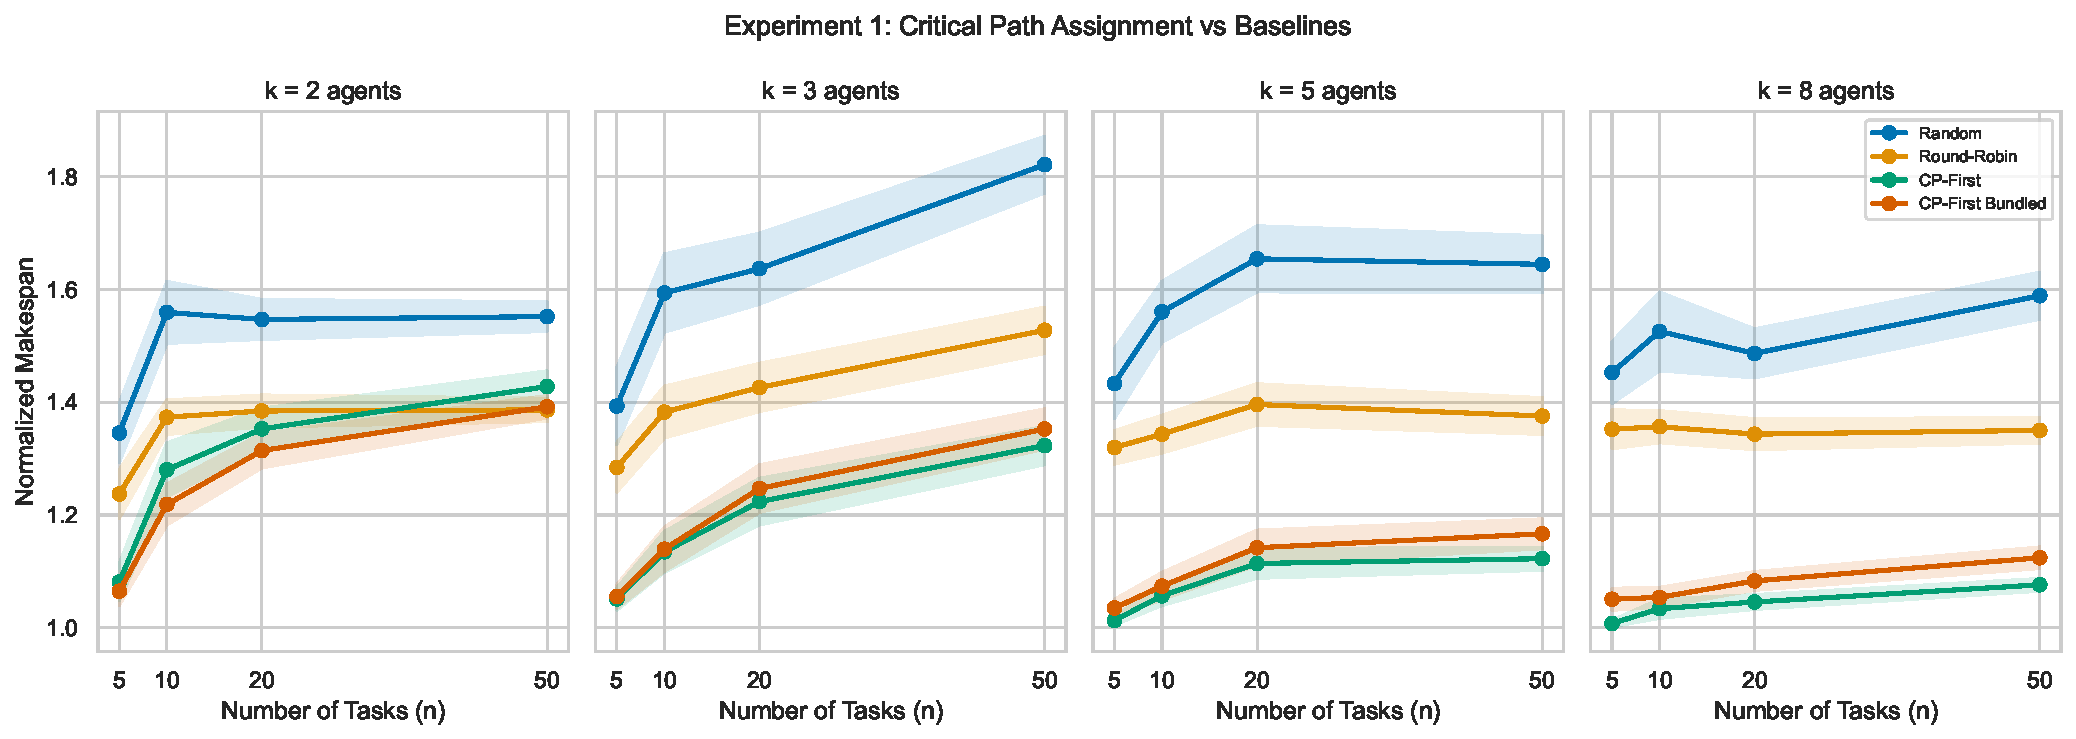
\includegraphics[width=\columnwidth]{figures/fig1_cp_assignment.pdf}
    \caption{Experiment 1: Normalized makespan across assignment strategies. CP-first consistently dominates round-robin and random, with 95\% CI bands.}
    \label{fig:exp1}
\end{figure}

\subsection{Experiment 2: Validator Placement}

\paragraph{Setup.} Linear chains of length $m \in \{3, 5, 7, 10\}$ (worst case for error compounding). Amplification factors $A_{ij} \sim \text{LogNormal}(\mu, \sigma)$ with mean 1.5 and standard deviation 0.5. Initial error $\epsilon_0 = 0.1$. 500 trials per configuration.

\paragraph{Conditions.} No validator, random placement, optimal single-validator placement (argmax interior prefix product), and two validators: $k_2$ = single-validator optimum, $k_1$ = prefix-product optimum in the sub-chain before $k_2$ (minimising rework in the prefix without changing final error).

\paragraph{Results (Figure~\ref{fig:exp2}).} Without validation, mean final error grows from 0.23 ($m=3$) to 3.84 ($m=10$), consistent with exponential accumulation (Proposition~\ref{prop:error}). Optimal single-validator placement (argmax interior prefix product) stabilizes final error to approximately 0.15 across all chain lengths---a 34\% reduction at $m=3$ growing to 96\% at $m=10$---because the prefix-product-maximizing interior position consistently leaves only the last CP edge in the post-validator suffix. For $m\geq 5$, optimal outperforms interior random placement by 38--82\% on final error (at $m=3$ both pick the only interior candidate). Two validators place $k_2$ at the single-validator optimum, yielding identical final error; their distinct benefit is in rework cost, which falls 80\% at $m=7$ and 51\% at $m=10$ relative to one validator. Note that optimal single-validator placement minimises final error but not rework, since it always places near the end of the chain; earlier or distributed placement (including random) can intercept more intermediate high-error tasks at the cost of a higher final error.

\begin{figure}[t]
    \centering
    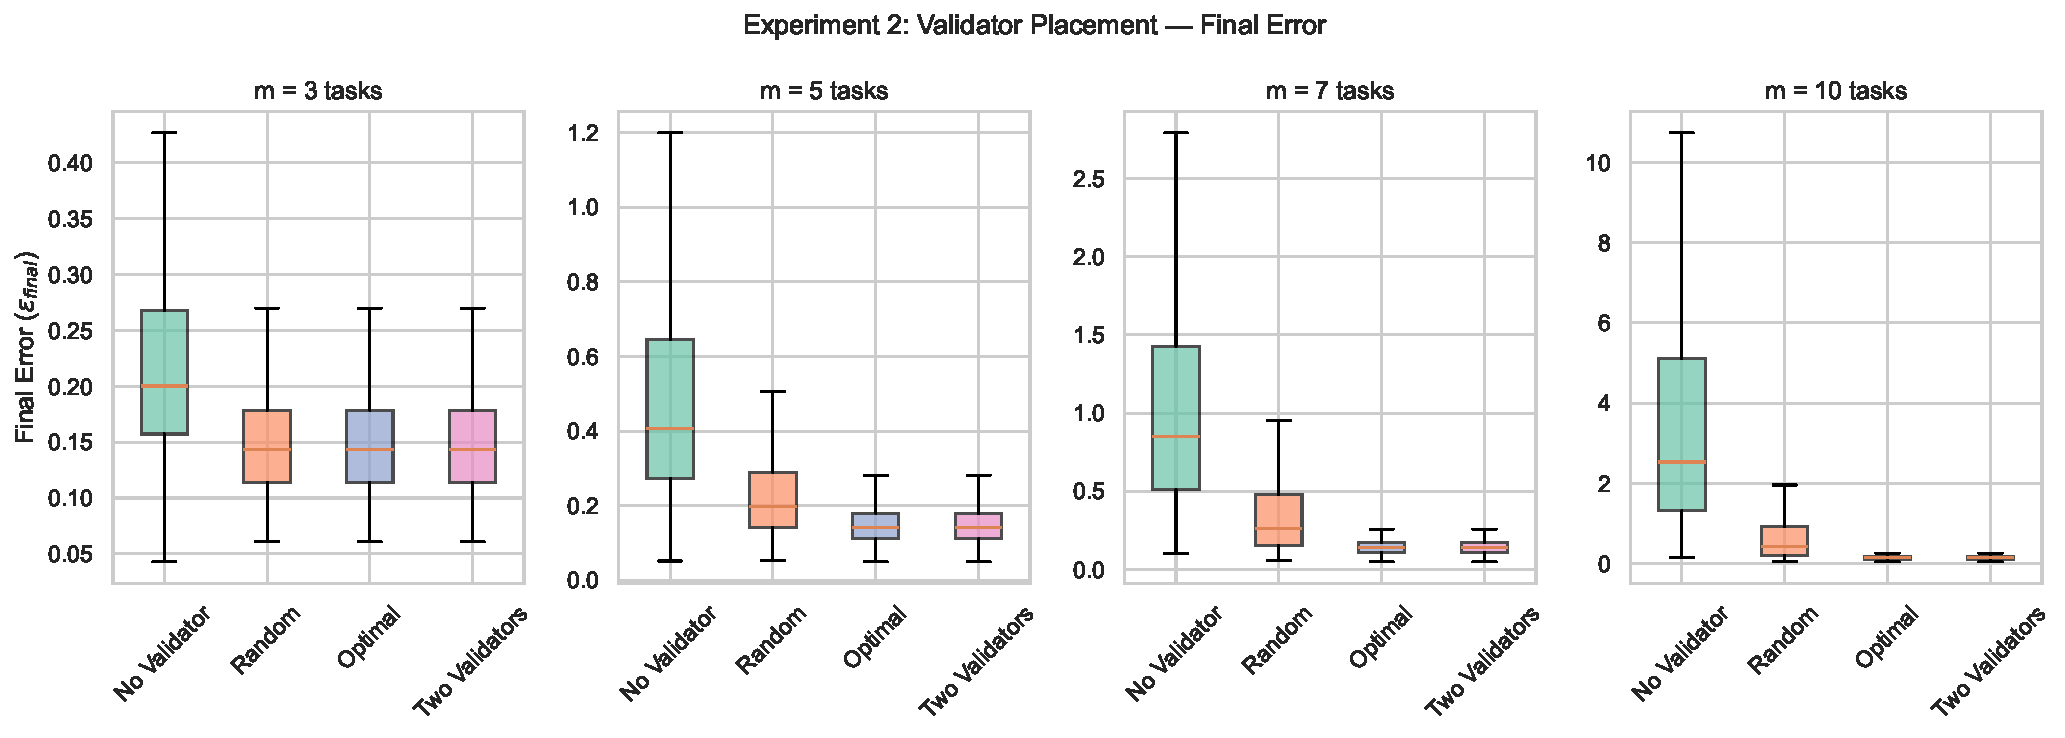
\includegraphics[width=\columnwidth]{figures/fig2_validator_error.pdf}
    \caption{Experiment 2: Final error (top row) and rework cost (bottom row) by validator strategy, stratified by chain length. Optimal and two-validator conditions are identical on final error; two validators reduce rework cost by 51--80\% at $m \geq 7$.}
    \label{fig:exp2}
\end{figure}

\subsection{Experiment 3: Optimal Agent Count}

\paragraph{Setup.} Fixed 7-task research pipeline DAG. Agent count swept over $k \in \{1, \ldots, 12\}$. Three coordination topologies: tree ($|G|=k-1$), pipeline ($|G|=k-1$), and all-to-all ($|G|=\binom{k}{2}$).

\paragraph{Results (Figure~\ref{fig:exp3}).} Total cost (makespan + overhead) exhibits the clearest U-shape for all-to-all topology, with empirical $N^*=2$ and analytical prediction $N^*_{\text{ana}} \approx 1.73$. The close agreement indicates that the cube-root scaling captures the dominant tradeoff once coordination grows quadratically. Tree topology tolerates one additional agent ($N^*=3$), while pipeline and all-to-all topologies both peak at $N^*=2$ because the 7-task DAG has width 3 but a long serial tail. This validates Proposition~\ref{prop:nstar} while also illustrating why the width-based practical bound is necessary.

\begin{figure}[t]
    \centering
    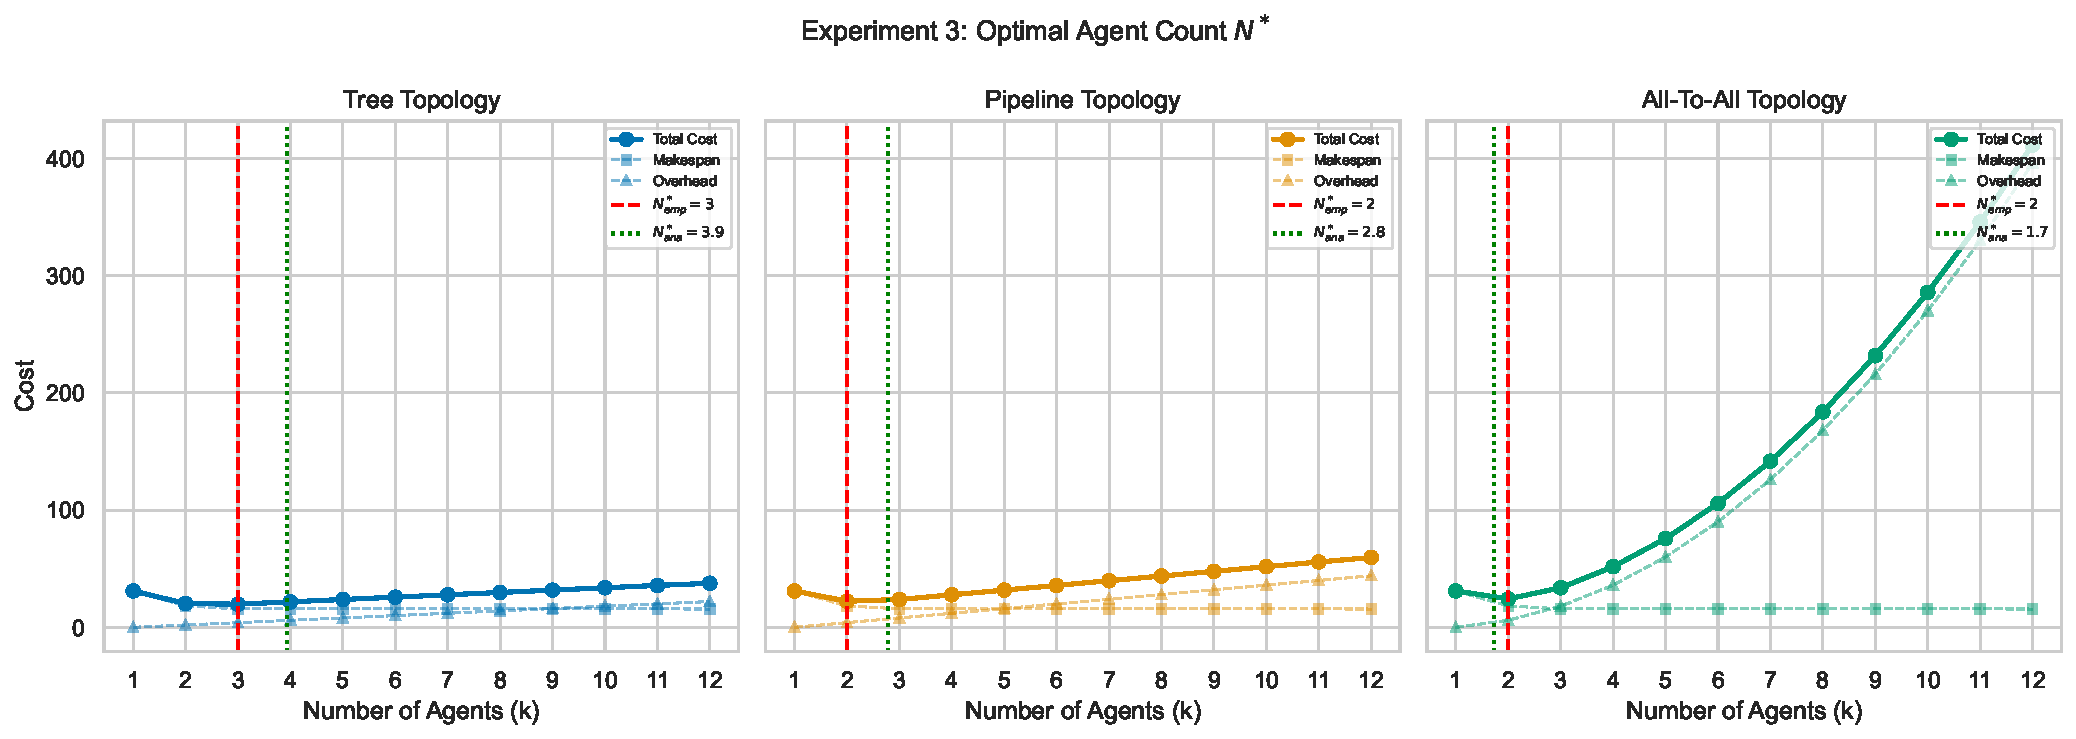
\includegraphics[width=\columnwidth]{figures/fig3_nstar.pdf}
    \caption{Experiment 3: Total cost vs.\ agent count for three coordination topologies. Vertical dashed lines mark empirical $N^*$.}
    \label{fig:exp3}
\end{figure}

\subsection{Experiment 4: Representation Format}

\paragraph{Setup.} Seven-task research pipeline with three inter-agent representation formats: \texttt{prose} ($C_{kj}=1.0$, error multiplier 1.4), \texttt{structured\_json} ($C_{kj}=0.6$, multiplier 0.9), and \texttt{compressed\_summary} ($C_{kj}=0.3$, multiplier 1.1). Base $A_{ij}$ swept over $[0.5, 3.0]$.

\paragraph{Results (Figure~\ref{fig:exp4}).} In the low-amplification regime, compressed summary is best up to approximately $A_{ij}^{base}=1.25$ because the reduced transfer cost outweighs its mild error amplification. Structured JSON overtakes it around $A_{ij}^{base}=1.5$ and widens the gap thereafter; at $A_{ij}^{base}=3.0$, it lowers total cost by about 15\% relative to compressed summary and by more than 40\% relative to prose. Prose is dominated throughout the practically relevant error-amplifying regime, confirming that representation is a first-order optimization variable rather than a serialization detail.

\begin{figure}[t]
    \centering
    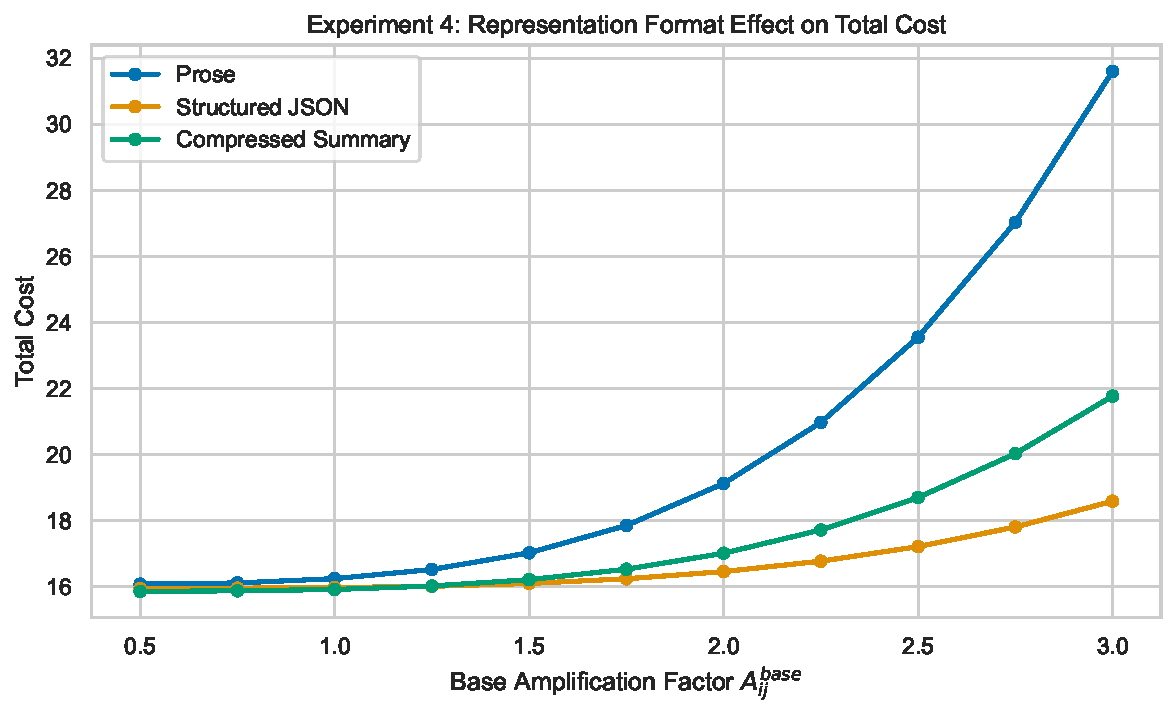
\includegraphics[width=\columnwidth]{figures/fig4_representation.pdf}
    \caption{Experiment 4: Total cost vs.\ base amplification factor for three representation formats. Structured JSON dominates in the error-amplifying regime.}
    \label{fig:exp4}
\end{figure}

\subsection{Experiment 4b: LLM Pilot Study of Representation Effects}

\paragraph{Setup.}
To ground the simulation results in real LLM behavior, we instantiate the same 7-task research pipeline DAG using the Anthropic Claude API (\texttt{claude-haiku-4-5}). The topic is \textit{``impact of sleep on athletic performance''}; tasks span literature review, data collection, problem framing, method design, implementation, evaluation, and paper writing. Each task prompt is prepended with the chosen format instruction (prose, structured JSON, or compressed bullet points) and dependent predecessor outputs are passed as context. Handoff quality is scored by a separate LLM judge call that returns $A_{ij} \in [0, 2]$ per directed edge; 1.0 indicates no change, below 1 indicates synthesis gain, above 1 indicates information loss.

\paragraph{Results (Figure~\ref{fig:exp4b}).}
Across the seven handoff edges, mean measured $A_{ij}$ values are 1.00 for prose, 1.20 for structured JSON, and 1.17 for compressed summary. Counterintuitively, prose achieves the lowest total cost (37.2 vs.\ 44.0 for both structured formats), driven primarily by faster generation latency: prose tasks complete in 5--8 s per step versus 8--10 s for constrained formats. However, prose also exhibits higher variance in $A_{ij}$---two handoffs score 0.3 (strong synthesis) while three score 1.3 (moderate loss), compared with the more uniform degradation profile of the other formats. On the critical path edges (Problem Framing $\to$ Method Design $\to$ Implementation $\to$ Evaluation $\to$ Paper Writing), the cumulative error products are 0.61, 1.76, and 2.43 for prose, structured JSON, and compressed summary respectively, suggesting that in this topic and model setting, prose can promote synthesis at certain boundaries while structured formats impose more consistent but moderately amplifying constraints.

\paragraph{Caveats.} This is a single run per format on one topic with the same model acting as both generator and judge, and wall-clock API latency is mixed into the cost metric alongside the theoretical overhead term. No confidence intervals are available. Results should be treated as indicative rather than conclusive.

These results carry two lessons for practitioners. First, representation format has a measurable and non-trivial effect on both latency and information fidelity in real LLM pipelines, consistent with Experiment~4's simulation prediction that format is a first-order optimization variable. Second, the relative ranking depends on topic and model: in settings where the base $A_{ij}$ is near 1.0 (as here), the latency component dominates and a lower-overhead format can win even if its error multiplier is slightly higher. At higher base amplification---as observed in the simulation sweep---structured JSON's multiplicative advantage grows and its cost ranking improves.

\begin{figure}[t]
    \centering
    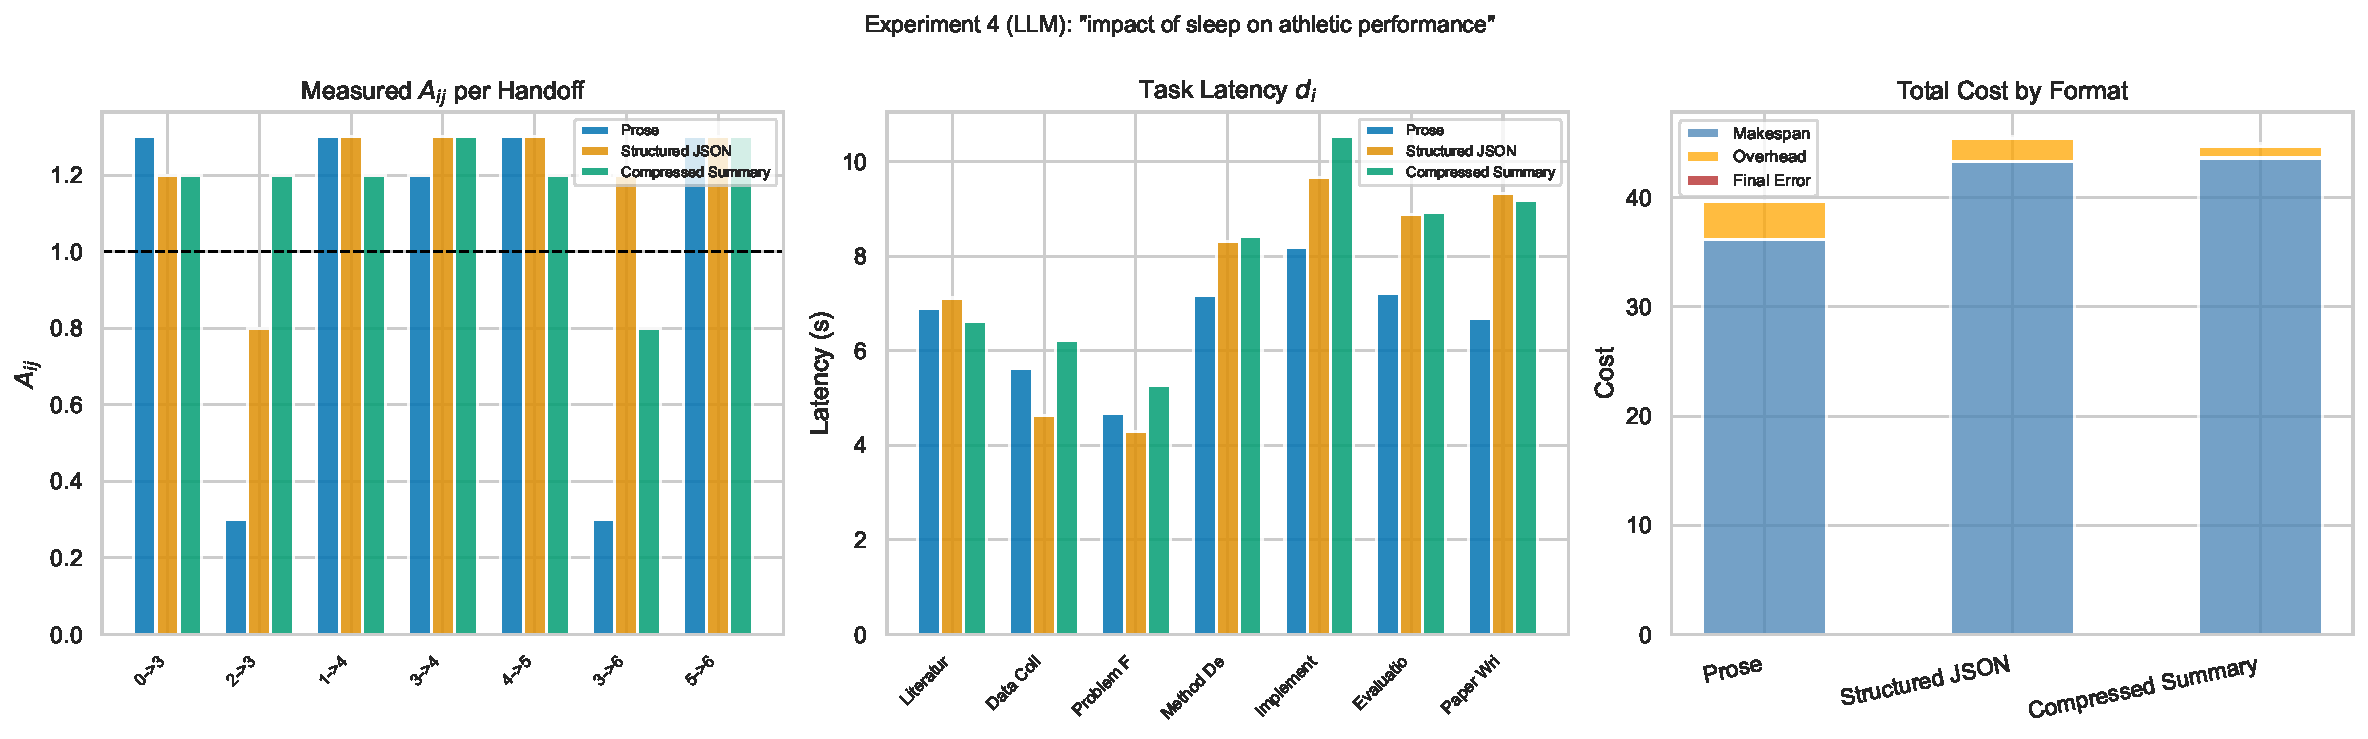
\includegraphics[width=\columnwidth]{figures/fig4_representation_llm.pdf}
    \caption{Experiment 4b (pilot, single run): Measured $A_{ij}$ per handoff (left), task latency per format (center), and total cost breakdown (right) on a real 7-task Claude pipeline. Results are indicative; no confidence intervals are available from a single run.}
    \label{fig:exp4b}
\end{figure}

\subsection{Experiment 5: Adaptive vs.\ Static Policy}

\paragraph{Setup.} Stochastic execution of the 7-task DAG over 1000 episodes. Durations follow $d_i \cdot \text{LogNormal}(0, 0.3)$. Tasks fail with probability $p_i$, doubling duration and resetting output. Amplification factors drift as $A_{ij}^{(t+1)} = A_{ij}^{(t)} + \mathcal{N}(0, 0.3)$, and we evaluate total cost in a coordination-aware regime with $(\alpha, \beta, \gamma) = (1.5, 1.0, 1.5)$.

\paragraph{Methods.} (i) \texttt{static\_naive}: round-robin, no validators, no replanning; (ii) \texttt{static\_optimized}: CP-first + optimal validator, no replanning; (iii) \texttt{adaptive}: replanning at each task completion; (iv) \texttt{adaptive\_with\_repr}: adaptive + representation selection.

\paragraph{Results (Figure~\ref{fig:exp5}).} The clearest benefit of closed-loop control is in the tail. Relative to \texttt{static\_naive}, the 95th-percentile episode cost drops from 69.95 to 45.25 for \texttt{static\_optimized}, to 45.01 for \texttt{adaptive}, and to 44.70 for \texttt{adaptive\_with\_repr}; mean cost follows the same ordering (48.50 $\rightarrow$ 28.50 $\rightarrow$ 28.25 $\rightarrow$ 28.05). Against the strong \texttt{static\_optimized} baseline, the mean gains are small because the 7-task DAG is narrow, so the right interpretation is robustness: adaptive control catches $A_{ij}$ drift before it compounds into late-stage rework. We report absolute dispersion and tail risk rather than normalized CV because optimization shrinks the mean faster than the spread.

\begin{figure}[t]
    \centering
    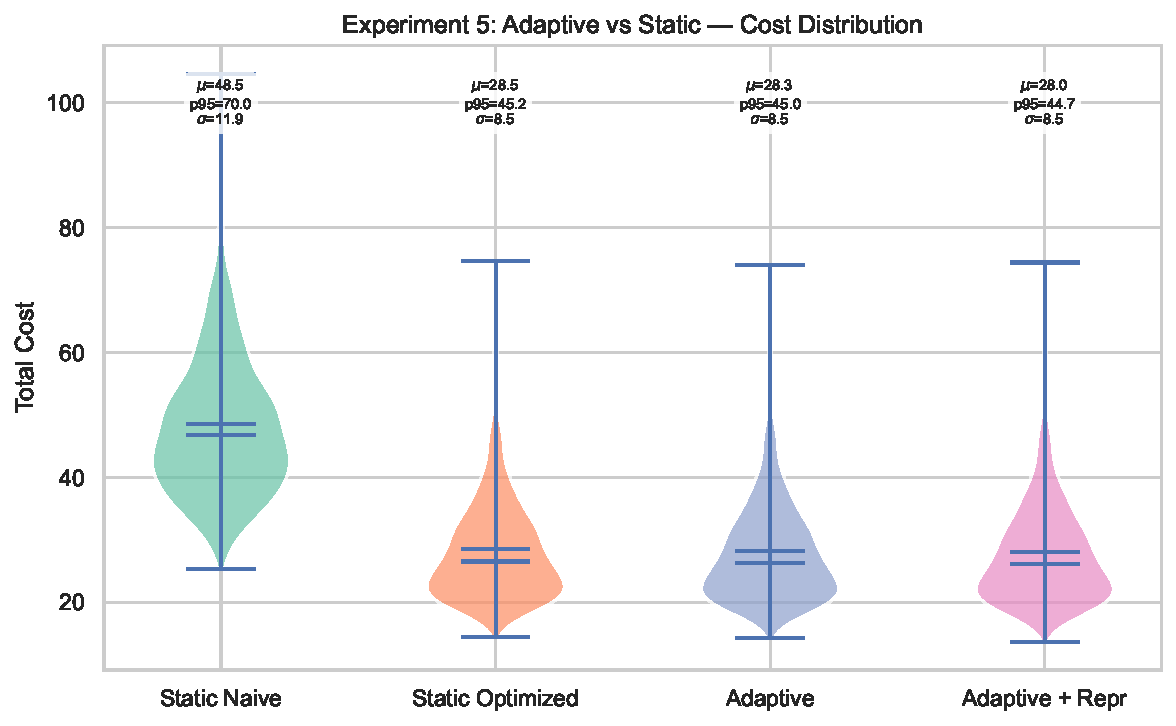
\includegraphics[width=\columnwidth]{figures/fig5_adaptive.pdf}
    \caption{Experiment 5: Total cost distributions. Adaptive policies reduce both mean and tail cost.}
    \label{fig:exp5}
\end{figure}

\begin{table}[t]
\centering
\caption{Stochastic controller comparisons on the 7-task DAG.}
\label{tab:controller_summary}
\scriptsize
\resizebox{\columnwidth}{!}{%
\begin{tabular}{lcccc}
\toprule
Controller & Mean & p95 & $\sigma$ & Addition \\
\midrule
Static naive & 48.50 & 69.95 & 11.91 & RR + prose \\
Static optimized & 28.50 & 45.25 & 8.50 & CP + validator \\
Adaptive & 28.25 & 45.01 & 8.49 & + replanning \\
Adaptive + repr & 28.05 & 44.70 & 8.53 & + format choice \\
Adaptive + proactive & 22.87 & 35.92 & 6.98 & + spec/stop/skip \\
\bottomrule
\end{tabular}
\hspace{0pt}}
\end{table}

\subsection{Experiment 6: Proactive Control Primitives}

\paragraph{Setup.} We study four stylized proactive controls using the same cost model as the main simulator. Speculative execution is evaluated on 6-task serial chains with hit rate $\rho \in [0.30, 0.95]$, structural predictability $q \in \{0.4, 0.7, 1.0\}$, wasted-work penalty $\lambda_s = 0.85$, and per-edge launch cost $c_s = 0.45$. Predictive early stopping sweeps observation fraction $t/d_i$ over the 7-task DAG using a noisy partial-quality predictor. Conditional DAG morphing decides whether a downstream verification task should be skipped from an observed quality score. Context pre-warming sweeps lead time $\tau$ for structured JSON and compressed-summary handoffs.

\paragraph{Results (Figure~\ref{fig:exp6}).} Speculative execution exhibits the clearest threshold behavior: the empirical crossover occurs near $\rho^* \approx 0.70$ for $q=0.4$, $\rho^* \approx 0.60$ for $q=0.7$, and $\rho^* \approx 0.55$ for $q=1.0$, closely matching Proposition~\ref{prop:speculation}. At the moderate-predictability setting $q=0.7$ with $\rho=0.8$, speculation reduces cost to $0.78\times$ the serial baseline; the strongest gains in the sweep appear only in the fully predictable regime $q=1.0$. Early stopping has a shallower optimum at $t/d_i \approx 0.55$, yielding a 2.6\% mean cost reduction; DAG morphing is stronger on this verification-heavy DAG, skipping the downstream check in 53\% of episodes and lowering total cost by 7.6\%. Pre-warming shows clean lead-time optima at $\tau^*=0.50$ for structured JSON and $\tau^*=0.40$ for compressed summaries, cutting expected handoff overhead by 17\% and 29\%. Speculation is the headline result on serial critical paths, while DAG morphing is strongest on verification-heavy tails.

\begin{figure}[t]
    \centering
    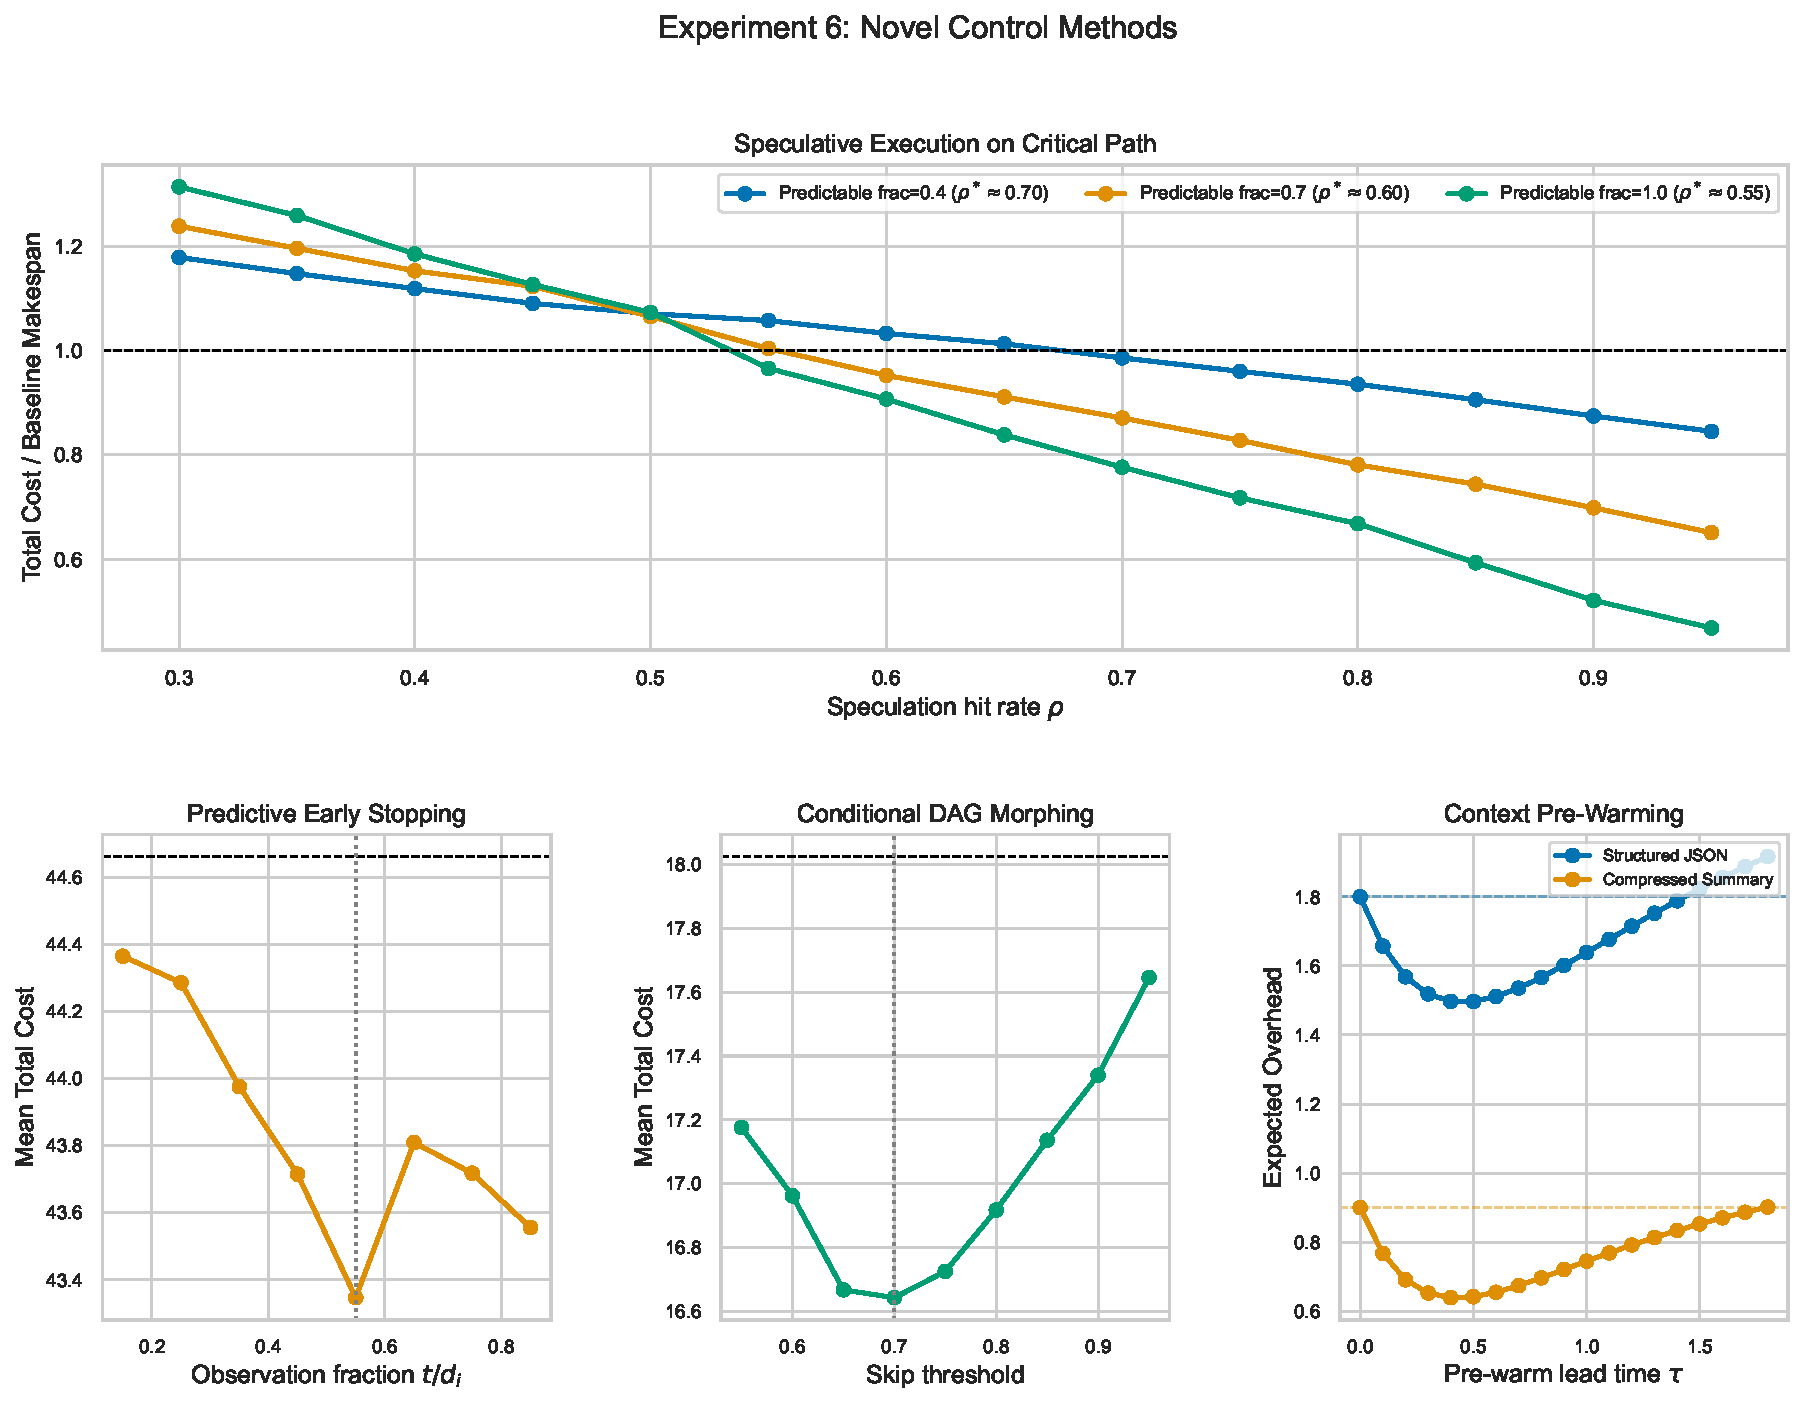
\includegraphics[width=0.98\columnwidth]{figures/fig6_novel_methods.pdf}
    \caption{Experiment 6: Proactive controls. Top: speculation threshold. Bottom: early stopping, DAG morphing, and pre-warming; dashed lines denote the no-control baseline in the lower panels.}
    \label{fig:exp6}
\end{figure}

\subsection{Experiment 7: Composed Proactive Controller}

\paragraph{Setup.} We return to the full stochastic 7-task setting from Experiment~5 and compare \texttt{adaptive\_with\_repr} against a heuristic stacked controller that adds speculative overlap ($q=0.7$), early-stop recovery ($t/d_i \approx 0.55$), and skip threshold 0.70 to the same adaptive backbone. We exclude pre-warming because at the current $\alpha$ its effect on total cost is small relative to the other three controls and including it would complicate per-primitive attribution without meaningfully changing the aggregate result. On the branching 7-task DAG, we apply Proposition~\ref{prop:speculation} locally to realized critical-path edge pairs; this is a conservative heuristic because parallel branches can absorb part of the mis-speculation cost. These parameters are selected from Experiment~6 on the same DAG family, so the result should be read as an optimistic upper bound rather than a zero-shot generalization claim.

\paragraph{Results.} The composed stack produces a clear end-to-end gain. Mean total cost drops from 28.05 to 22.87 and the 95th percentile falls from 44.70 to 35.92 (Table~\ref{tab:controller_summary}), while standard deviation shrinks from 8.53 to 6.98. Averaged over episodes, speculative overlap contributes 3.75 units of makespan reduction, conditional skipping 2.48, and early stopping 1.13; the skip gate fires in 49.4\% of episodes. This is not yet a fully integrated proactive controller, but it shows that the strongest proactive controls remain useful when stacked on the reactive backbone rather than only when studied in isolation.

% ─────────────────────────────────────────────────────────────────────────────
\section{Related Work}
\label{sec:related}

\paragraph{LLM Agent Frameworks.}
ReAct \citep{yao2023react} introduced interleaved reasoning and acting for single agents. Multi-agent extensions include MetaGPT \citep{hong2023metagpt}, which assigns roles to agents in a software development pipeline, AutoGen \citep{wu2023autogen}, which enables multi-turn conversations between agents, and CAMEL \citep{li2023camel}, which studies communicative agent collaboration. AgentBench \citep{liu2023agentbench} and AgentVerse \citep{chen2024agentverse} provide evaluation frameworks. More recent orchestration work is closer to our setting: VMAO \citep{zhang2026vmao} combines DAG execution with verifier-driven replanning, Flash-Searcher \citep{qin2026flashsearcher} uses DAG-based parallel execution with dynamic workflow refinement, and evolving orchestration \citep{dang2025evolving} learns a dynamic controller for agent sequencing. These works address orchestration directly, but they do not expose handoff representation format, validator placement, and task assignment as a single joint optimization objective.

\paragraph{Communication and Coordination Structure.}
Graph-of-Agents \citep{yun2026goa} shows that graph structure and directed message passing can improve multi-agent collaboration, while the LACP position paper \citep{li2025lacp} argues that protocol design should be treated as infrastructure rather than an implementation detail. Our work is complementary to this line: rather than proposing a universal communication standard, we focus on the systems question of when a handoff should occur, how much it should cost, and which representation makes that handoff safest.

\paragraph{Multi-Agent Reinforcement Learning.}
MARL methods such as QMIX \citep{rashid2020qmix} and MADDPG \citep{lowe2017multi} learn coordination policies through interaction. Our work differs in assuming a known task DAG structure, enabling analytical results rather than requiring sample-intensive training. Reflexion \citep{shinn2023reflexion} introduces verbal reinforcement for single agents but does not address multi-agent coordination.

\paragraph{DAG Task Scheduling.}
Classical results on multiprocessor scheduling \citep{graham1966bounds, coffman1972optimal} establish that list scheduling achieves $\leq 2$ approximation for makespan minimization. The HEFT algorithm \citep{topcuoglu2002heft} extends this to heterogeneous processors with communication costs. Distributed systems like Spark \citep{zaharia2010spark} and YARN \citep{vavilapalli2013yarn} implement DAG-aware scheduling. Our work extends this line by incorporating error propagation and representation-dependent overhead as first-class optimization variables, then adding proactive controls whose trigger condition is semantic uncertainty rather than processor occupancy alone.

\paragraph{Error Propagation in Pipelines.}
The hidden technical debt framework \citep{sculley2015hidden} identifies cascading failures in ML pipelines. Data management challenges \citep{polyzotis2017data} highlight quality propagation. Our error amplification model ($A_{ij}$) formalizes these concerns within the scheduling framework.

% ─────────────────────────────────────────────────────────────────────────────
\section{Discussion and Conclusion}
\label{sec:discussion}

\paragraph{Key Insight.}
The dominant bottleneck in multi-agent systems is not compute but \emph{interfaces}: the points where one agent's output becomes another's input. Error amplification at these boundaries ($A_{ij}$) compounds multiplicatively along execution paths, making it the primary driver of end-to-end quality degradation. Once interfaces are exposed as controllable objects, the orchestrator can act both reactively and proactively: it can validate or re-route after observing drift, but it can also speculate, stop early, skip redundant work, or pre-warm future handoffs before the full cost of a bad boundary is paid.

\paragraph{Limitations.}
Our model assumes $A_{ij}$ and the proactive predictors can be estimated or measured, but in this paper they are hand-specified in simulation and only lightly probed through a single-run LLM pilot. The empirical section should therefore be read as testing a systems hypothesis rather than conclusively validating a deployed orchestration mechanism. In particular, the current experiments do not yet show that intermediate handoff-risk estimates predict final failure on real workloads, nor that acting on those estimates improves objective benchmark outcomes. Experiment~7 addresses composition through a heuristic overlay whose parameters are selected on the same DAG family rather than through a fully integrated joint controller. The cube-root scaling of $N^*$ is idealized, and the adaptive policy uses greedy replanning rather than solving the full MDP.

\paragraph{Why gains over a strong baseline are modest.}
On the 7-task pipeline, CP-first assignment already matches the best available makespan on most episodes because the DAG width is only 3 and the serial tail dominates. Experiment~5 should therefore be read as refinement of a strong initial plan rather than wholesale schedule replacement: the closed-loop controller primarily improves interface decisions (validator placement and representation choice) once uncertainty resolves. The larger 11--20\% makespan gains in Experiment~1 appear when the DAG exposes more parallelizable structure, which is precisely the regime where assignment policy has more room to reshape execution. Experiment~6 shows a complementary regime: proactive controls matter most when they can attack serial waiting directly, especially on narrow critical paths or verification-heavy tails where reactive replanning arrives too late.

\paragraph{External validity path.}
The next empirical step is a real-trace calibration and intervention study. For each handoff edge, the controller should estimate $\hat{A}_{ij}=P(\text{downstream failure}\mid\text{handoff state})$ from concrete signals such as visible unit-test deltas, static-analysis warnings, schema validity, validation-score changes, runtime anomalies, LLM judge scores, and executor confidence. First, passive traces should test whether $\hat{A}_{ij}$ predicts final failure using AUROC, AUPRC, Brier score, and calibration curves. Then thresholds should be frozen and the risk-aware controller compared against single-agent, static-DAG, round-robin multi-agent, and risk-blind adaptive baselines under equal cost and latency budgets. SWE-bench Verified and MLE-bench are the strongest first targets because they provide objective software-engineering and ML-engineering outcomes; WfCommons/WfBench is the right non-LLM follow-up because it separates the scheduling contribution from LLM-specific uncertainty. WorkArena, TheAgentCompany, and tau-bench are useful transfer tests once the core calibration and intervention results are established.

\paragraph{Future Work.}
Promising next steps are learning $A_{ij}$ models and proactive predictors from execution traces, validating the controls on real benchmark pipelines with held-out final evaluators, testing cross-benchmark generalization of fixed thresholds, and extending the framework to hierarchical DAGs where subtask decomposition is itself a decision variable.

\paragraph{Conclusion.}
We have formalized multi-agent coordination as constrained DAG scheduling with error propagation, derived analytical results that explain when and why current approaches fail, and proposed an adaptive controller augmented with proactive control primitives. The resulting picture is broader than reactive replanning alone: reliable multi-agent systems should optimize not just who does each task and how outputs are validated, but also when dependent work can safely begin early, when failing work should be stopped, when redundant work can be pruned, and when future handoffs should be prepared in advance.

% ─────────────────────────────────────────────────────────────────────────────
\bibliographystyle{plainnat}
\bibliography{refs}

\end{document}
